\section{Datasheet}
\label{app:datasheet}
\textbf{Motivation.} IdCon measures whether a system returns the consensus diagnosis of a requirement pattern over all admissible embeddings, and at what cost. It was created by the authors; no external funding body shaped its content.

\textbf{Composition.} Each instance is a task: a pattern graph with roles, a host graph with entity coordinates, optional anchors, metric edges and unary domains, checked roles with $S/U/V$ observation tables, and a reference outcome in \{\Sat, \Vio, \Unk, \Emp\}. Tasks are grouped by ancestor (one pattern--host pair). IdCon-Hard has 72 ancestors and 504 tasks, IdCon-Hard-X \hardxAncestors{} and \hardxTasks{}, IdCon-HPRD 100 and 200, IdCon-HPRD-X 96 and 192, IdCon-Cite \citeAncestors{} and \citeTasks{}; the held-out IdCon-HPRD-H has 100 and 200 and IdCon-Hard-H 12 and \hardhTasks{}. Tasks without a determined reference are released as \textsc{Unassessed} and excluded from scoring. No instance contains personal information.

\textbf{Collection process.} The synthetic suites are produced by a seeded generator from six NetworkX random-graph families; patterns are extracted by seeded BFS; no solver is called during generation and no instance is selected or rejected by solver outcome. The HPRD suites import the data graph and query graphs unchanged from Sun and Luo and from the CEMR artifact; IdCon-Cite imports Cora and PubMed unchanged from Planetoid and extracts queries by seeded random walks. Only the checked-role choice and the observation rule are added.

\textbf{Preprocessing.} Host graphs are relabelled to contiguous integers; Cora and PubMed edges are made undirected, self-loops dropped, and the few unlabelled vertices removed. Synthetic coordinates are integer grid points with a per-entity offset below $10^{-3}$ of the length tolerance so that anchors are unique.

\textbf{Uses.} Evaluating exact and approximate consensus solvers, studying when first-match diagnosis fails, and testing adapters that turn subgraph engines into certain-answer engines. Labels are environment-independent; timings are not.

\textbf{Distribution and licences.} Code MIT; our generated data, references and predictions CC BY 4.0. HPRD is free for academic, non-commercial use and commercial users need a licence from its maintainers; the CEMR query files carry no licence; Planetoid is MIT-licensed and Cora and PubMed should be cited as their creators ask. None of these is redistributed: fetch scripts pin the upstream commits, and task files built from them are generated locally and inherit their terms. The patched LAD2025 sources are CeCILL-B.

\textbf{Maintenance.} The corresponding author maintains the repository; \archiveSentence. Errata and new results are added as new records; frozen records are never edited. Held-out predictions are scored on request.

\section{Stages, Amendments and Deviations}
\label{app:registration}
\textbf{Stage-1 design record.} After input generation and before any timed inference or reference computation, a local hash-stamped record fixed the IdCon-Hard seed, factors, scenarios, methods, budget, scoring and reference procedure, with SHA-256 hashes of sources, binaries, manifest, inputs and construction maps; IdCon-HPRD had its own record before inference. Neither was publicly timestamped. Tier sizes came from a pilot on six cells with a different seed.

\textbf{Amendment 1 (stage 1).} \textsf{decoy\_s} (checked roles $V$, decoys $S$) is decided by the observation tables: an identity has state $S$ only if every checked role lands on an $S$ entity, and decoys reach only some checked roles, so every reference is \Vio. It was kept in the scored set as a control, and \textsf{focal\_v} was added before any of its inference or references.

\textbf{Amendment 2 (stage 1).} Some constrained 8,192-entity references were unresolved after the LAD/Glasgow/CP-SAT procedure. The amendment let EG-ICAF, a consensus solver of the authors, settle state queries; it was made while timed inference was running and after an interim look at partial predictions. Three tasks were settled that way (re-settled without it in stage~2).

\textbf{Amendment 3 (stage 1, post hoc arm).} After scoring, default Glasgow had answered no IdCon-HPRD run; profiling showed about 1.4~s per call in its supplemental-graph preprocessing of the gadget-enlarged target. The \texttt{-{}-staged} arm was added with the same encoding, driver and budget, and is marked $^\dagger$ on IdCon-Hard and IdCon-HPRD.

\textbf{Stage-2 design record and Amendment 4.} Written before any stage-2 run (\path{experiment/results/revision_r1/design.json}). It dropped a stage-1 suite of the authors' own construction (IdCon-Core) and the authors' solvers EG-ICAF and LAD-SV from the benchmark, re-settled the Amendment-2 tasks, re-queried every unconfirmed negative, and added the tool baselines, IdCon-HPRD-X, IdCon-HPRD-H, the 10~s reruns, the overhead and embedding-count measurements, and the stage-2 analyses. Dropping them was decided after the stage-1 results were known; the two solvers' frozen results are in Table~\ref{tab:legacy}: EG-ICAF answers \legEgCorrect{} of 1,008 IdCon-Hard runs at 2\,s (PAR-2 \legEgPar~ms) and LAD-SV \legSvCorrect{} (\legSvPar~ms), both without a wrong certified answer. They are not ranked because they are unpublished methods of the authors.

\textbf{Stage-2 deviations.} (i) The stage-1 Glasgow binary did not record its source commit; stage~2 rebuilt commit \texttt{01ef6ca}. (ii) Proof logging is not used for Glasgow: its \texttt{-{}-prove} rejects labelled inputs. (iii) Enum-Glasgow builds metric gadgets in Python without interruption, so some runs overran the budget (scored as unanswered). (iv) The VM restarted at about 20:30~UTC during the embedding counts; the orchestrator resumed from the records. (v) The two concurrent reference re-check shards were killed three times by the out-of-memory killer (about 3~GB per CP-SAT or Glasgow query on 8,192-entity hosts); the re-check was finished serially and then per task with a 6.5~GB limit; it overlapped in time with some timed stage-2 jobs on the other vCPU. All are logged in \path{orchestrate.log}.

\textbf{Stage-3 design record and Amendment 5.} Written before any stage-3 run, any generation of the stage-3 suites and any stage-3 reference (\path{experiment/results/revision_r2/design.json}). It fixes IdCon-Hard-X, IdCon-Hard-H and IdCon-Cite, the SAT baseline, the 2/10/60\,s runs, the independent check, the overhead decomposition, the calibration and the stage-3 analyses; Amendment~5 lists the post hoc analyses (Table~\ref{tab:registration}). The stage-2 primary analysis (504 IdCon-Hard tasks with \textsf{decoy\_s}) stays primary. Pilots used seeds 777002--777005 outside every suite; on 10 pilot tasks the independent check agreed with the reference procedure.

\textbf{Stage-3 deviations.} (i) Stage~3 ran on a different 2-vCPU VM (calibration in Section~\ref{sec:protocol}). (ii) LAD2025 crashes with the default 8\,MB stack on 16,384-entity hosts; stage-3 jobs run with an unlimited stack. (iii) The orchestrator was restarted once to stop an executor from idling while a memory-heavy job ran (the scheduler change is in the repository), and once after the VM restarted; runs in flight were not recorded and were rerun from the records. (iv) The machine also served light interactive work (editing, compiling) during the timed jobs. (v) The machine has 8\,GB of memory. On 16,384-entity hosts the out-of-memory killer ended Glasgow runs (recorded as runtime errors, Table~\ref{tab:errors}), Glasgow corroboration queries of the reference builder (logged as no evidence, which is why few IdCon-Hard-X negatives are corroborated), and six times a whole Python job: the two 60\,s IdCon-Hard-X jobs, one IdCon-Hard-H reference shard (twice) and the independent check (three times). From 12:14~UTC a guard made the killer prefer solver processes; from 14:33~UTC a 12\,GB swap file was available, and the remaining memory-heavy jobs (the 60\,s IdCon-Hard-X runs among them) ran one at a time. Interrupted jobs resumed from their records; runs in flight were not recorded.

\textbf{Amendments 6 and 7 (stage 3, during the runs).} After 4 of the registered independent-check tasks had finished (two unresolved after 687 and 1,222\,s), Amendment~6 lowered the limits to 120\,s per solve and 300\,s per proof check, ordered the check IdCon-Cite first, and replaced the 72 IdCon-Hard-X tasks by one seeded task per ancestor, because the registered workload would have taken well over a day on 2 vCPUs. After the IdCon-Hard-X references showed that most of their negatives rest on one engine, Amendment~7 added every IdCon-Hard-X task with such a negative. Both were written before the tasks they add were checked (\path{amendment_6.json}, \path{amendment_7.json}); a lower limit can turn an agreement into \emph{unresolved} but cannot create a disagreement.

\begin{table*}[t]
\caption{Status of every reported analysis. S1-reg / S2-reg / S3-reg: fixed in the design record of stage 1, 2 or 3 before any run of that stage; S1-post / S2-post: decided after results of that stage; S3-post: decided after results and recorded in Amendment~5 of the stage-3 record; S3 A6/A7: amendments made during the stage-3 runs. Known: whether results on the same suite were known when the analysis was fixed; an analysis fixed before a stage's runs but after earlier results on the same data protects less than a registration before any result.}
\label{tab:registration}
\centering\footnotesize
\begin{tabular}{p{0.52\textwidth}llp{0.20\textwidth}}
\toprule
Analysis & Status & Known & Where\\
\midrule
2\,s comparison of LAD, Glasgow, CP-SAT, Trad-CP, First-match on Hard and HPRD (correct, wrong, PAR-2) & S1-reg & no & Table~\ref{tab:main}\\
Reference procedure (LAD2025, Glasgow confirmation, CP-SAT fallback) & S1-reg & no & Section~\ref{sec:protocol}\\
\textsf{focal\_v} added; \textsf{decoy\_s} kept in the scored set as a control & S1 (A1) & partly & Section~\ref{sec:bench}\\
Glasgow-staged on Hard and HPRD & S1-post (A3) & yes & Table~\ref{tab:main} ($^\dagger$)\\
Scenario and metadata priors; correct runs by label; 0.5/1\,s budgets; family and scenario tables; confirmed-subset results & S1-post & yes & Tables~\ref{tab:suites}, \ref{tab:labels}, \ref{tab:budget}, \ref{tab:scenario}, \ref{tab:family}, \ref{tab:refs}\\
VBS over the stage-1/2 registered methods (Glasgow-staged excluded) & S1-post & yes & Section~\ref{sec:exact}\\
Removal of IdCon-Core, EG-ICAF and LAD-SV (Amendment 4) & S2-reg & yes & Appendix~\ref{app:registration}\\
Enum-Glasgow, Enum-VF2, ASP-cautious on Hard and HPRD; all methods on HPRD-X; HPRD-H references & S2-reg & Hard, HPRD: yes & Tables~\ref{tab:main}, \ref{tab:labels}\\
Reference re-check of unconfirmed negatives; re-settling the Amendment-2 tasks & S2-reg & yes & Section~\ref{sec:refquality}, Table~\ref{tab:refs}\\
10\,s reruns of unanswered pairs; per-call overhead on HPRD & S2-reg & yes & Section~\ref{sec:budget}, Table~\ref{tab:budget}\\
First-match errors by reference label; embedding counts; soundness gate and PAR-10w; stratum bootstrap; learned prior; symmetry & S2-reg & Hard, HPRD: yes & Sections~\ref{sec:firstmatch}--\ref{sec:prior}\\
Repeat agreement of outcomes & S2-post & yes & Section~\ref{sec:limits}\\
IdCon-Hard-X, IdCon-Hard-H, IdCon-Cite: generation, runs at 2/10/60\,s, references, priors & S3-reg & no & Tables~\ref{tab:suites}, \ref{tab:newsuites}\\
SAT baseline on every suite & S3-reg & no & Tables~\ref{tab:main}, \ref{tab:newsuites}\\
60\,s reruns on IdCon-Hard; VBS at 2, 10 and 60\,s with and without Glasgow-staged & S3-reg & 2/10\,s: yes & Section~\ref{sec:budget}\\
Independent check with DRAT proofs; overhead decomposition on Hard; machine calibration & S3-reg & references: yes & Table~\ref{tab:idcheck}, Section~\ref{sec:budget}\\
Independent check: lower limits, IdCon-Cite first, one IdCon-Hard-X task per ancestor (Amendment 6); every single-engine IdCon-Hard-X negative (Amendment 7; fixed after 4 check results and the Hard-X references) & S3 A6/A7 & partly & Table~\ref{tab:idcheck}, Appendix~\ref{app:registration}\\
Disclosure of EG-ICAF and LAD-SV; \textsf{decoy\_s} and table-decided sensitivity; automorphism-corrected counts; ``not distinguishable'' strata; runtime errors; prior overlap & S3-post & yes & Tables~\ref{tab:legacy}, \ref{tab:sensitivity}, \ref{tab:errors}; Sections~\ref{sec:firstmatch}, \ref{sec:prior}\\
\bottomrule
\end{tabular}
\end{table*}


\textbf{Timing.} All methods run in one Python driver (3.10 in stages 1--2, 3.13 in stage 3) on a 2-vCPU Linux VM, single-threaded, in a randomized method order per task and repeat, with two executors pinned to one vCPU each.

\begin{table}[t]
\caption{The authors\textquotesingle{} own unpublished solvers EG-ICAF and LAD-SV, run in stage~1 and not part of the benchmark (Amendment~4), from the frozen stage-1 records scored against the final references. They are not ranked; they show that the headroom left by the benchmarked methods is not a lower bound on what exact methods can do. VBS unsolved: runs that no sound method answers, over the stage-1 and stage-2 methods / with EG-ICAF / with both.}
\label{tab:legacy}
\centering\footnotesize
\setlength{\tabcolsep}{3pt}
\begin{tabular}{lrrr rrr}
\toprule
 & \multicolumn{3}{c}{IdCon-Hard (1,008 runs)} & \multicolumn{3}{c}{IdCon-HPRD (400 runs)}\\
\cmidrule(lr){2-4}\cmidrule(lr){5-7}
Method & Correct & Wrong & PAR-2 & Correct & Wrong & PAR-2\\
\midrule
LAD & 725 & 0 & 1,635 & 389 & 0 & 1,036\\
EG-ICAF & 861 & 0 & 874 & -- & -- & --\\
LAD-SV & 799 & 0 & 1,352 & 400 & 0 & 971\\
\midrule
VBS unsolved & \multicolumn{3}{c}{186 / 34 / 29} & \multicolumn{3}{c}{0 / 0 / 0}\\
\bottomrule
\end{tabular}
\end{table}

\begin{table}[t]
\caption{IdCon-Hard sensitivity (Amendment~5, post hoc): correct runs and ancestor-equal PAR-2 (ms) on all 504 tasks (registered analysis), without the \textsf{decoy\_s} control (432), and without the 113 tasks whose label the observation tables decide up to the existence of an identity (two states excluded by the tables in a scenario whose construction embedding is admissible; 70 of them \textsf{decoy\_s}).}
\label{tab:sensitivity}
\centering\footnotesize
\setlength{\tabcolsep}{2.4pt}
\begin{tabular}{lrr rr rr}
\toprule
 & \multicolumn{2}{c}{All (1,008 runs)} & \multicolumn{2}{c}{No \textsf{decoy\_s} (864)} & \multicolumn{2}{c}{Non-trivial (782)}\\
\cmidrule(lr){2-3}\cmidrule(lr){4-5}\cmidrule(lr){6-7}
Method & Correct & PAR-2 & Correct & PAR-2 & Correct & PAR-2\\
\midrule
LAD & 725 & 1,635 & 594 & 1,757 & 517 & 1,857\\
Glasgow & 562 & 2,113 & 460 & 2,209 & 398 & 2,288\\
Glasgow-staged & 651 & 1,740 & 534 & 1,846 & 464 & 1,940\\
CP-SAT & 321 & 2,998 & 279 & 2,982 & 254 & 2,966\\
Trad-CP & 214 & 3,347 & 187 & 3,332 & 165 & 3,320\\
Enum-Glasgow$^\ast$ & 88 & 3,688 & 82 & 3,659 & 82 & 3,626\\
Enum-VF2$^\ast$ & 14 & 3,951 & 14 & 3,943 & 14 & 3,937\\
ASP-cautious$^\ast$ & 15 & 3,968 & 14 & 3,965 & 12 & 3,964\\
SAT$^\ddagger$ & 240 & 3,378 & 206 & 3,372 & 182 & 3,369\\
\midrule
First-match & 626 & 1,901 & 493 & 2,078 & 417 & 2,189\\
\bottomrule
\end{tabular}
\end{table}

\begin{table}[t]
\caption{Runs that ended in a runtime error (scored as unanswered), over all records of each suite. Enum-Glasgow errors on IdCon-Hard are processes killed by the operating system for memory (exit $-9$).}
\label{tab:errors}
\centering\footnotesize
\setlength{\tabcolsep}{3pt}
\begin{tabular}{lrrrrr}
\toprule
Method & Hard & HPRD & HPRD-X & Hard-X & Cite\\
\midrule
LAD & 0/1252 & 0/406 & 0/384 & 0/186 & 0/480\\
Glasgow & 0/1008 & 0/600 & 0/384 & 20/144 & 0/384\\
Glasgow-staged & 55/1344 & 0/452 & 0/384 & 26/183 & 35/515\\
CP-SAT & 0/1378 & 0/408 & 0/384 & 0/144 & 0/514\\
Trad-CP & 0/1008 & 0/400 & 0/384 & -- & 0/384\\
Enum-Glasgow$^\ast$ & 166/1468 & 0/493 & 0/384 & 0/144 & 0/384\\
Enum-VF2$^\ast$ & 0/1008 & 0/400 & 0/384 & -- & 0/384\\
ASP-cautious$^\ast$ & 0/1008 & 0/400 & 0/384 & -- & 0/467\\
SAT$^\ddagger$ & 0/1008 & 0/400 & 0/384 & 0/214 & 0/447\\
First-match & 0/1008 & 0/400 & 0/384 & 0/144 & 0/384\\
\bottomrule
\end{tabular}
\end{table}


\begin{figure*}[t]
\centering
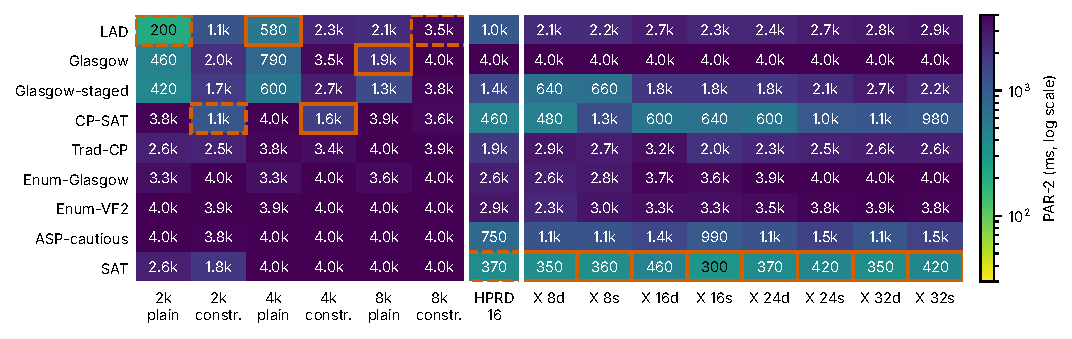
\includegraphics[width=\textwidth]{figures/fig3_strata.pdf}
\caption{Ancestor-equal PAR-2 (ms) per stratum: IdCon-Hard by host tier and variant, IdCon-HPRD, and IdCon-HPRD-X by query size and density. Boxes mark the best certified method per column (on Hard and HPRD, Glasgow-staged is a post hoc arm and is never boxed); a dashed box marks a column whose best and second-best methods are not distinguishable (bootstrap interval includes 0).}
\label{fig:strata}
\end{figure*}

\begin{table*}[t]
\caption{IdCon-Hard by stratum: ancestor-equal PAR-2 in ms (correct runs) and, last row, the bootstrap probability that the best certified method has the lowest PAR-2 with the 95\% interval of its difference to the runner-up (10,000 ancestor resamples, stratified by family; 12 ancestors per stratum, 2 per family). Best certified method in bold; $^{\circ}$the interval includes 0, so the best and second-best methods are not distinguishable. P(best) is the share of resamples in which the method is best, a stability measure rather than a probability of being best.}
\label{tab:strata-hard}
\centering\scriptsize\setlength{\tabcolsep}{2.5pt}
\begin{tabular}{lrrrrrr}
\toprule
Method & 2k plain & 4k plain & 8k plain & 2k constr. & 4k constr. & 8k constr.\\
\midrule
LAD & \textbf{196 (168)} & \textbf{580 (165)} & 2,108 (117) & 1,121 (147) & 2,306 (91) & \textbf{3,500 (37)}\\
Glasgow & 458 (154) & 789 (152) & \textbf{1,877 (120)} & 2,007 (104) & 3,548 (32) & 4,000 (0)\\
Glasgow-staged$^\dagger$ & 418 (154) & 602 (154) & 1,302 (138) & 1,693 (113) & 2,672 (73) & 3,751 (19)\\
CP-SAT & 3,842 (8) & 3,954 (2) & 3,925 (4) & \textbf{1,086 (142)} & \textbf{1,607 (137)} & 3,576 (28)\\
Trad-CP & 2,618 (76) & 3,758 (16) & 3,957 (2) & 2,481 (80) & 3,374 (33) & 3,895 (7)\\
Enum-Glasgow$^\ast$ & 3,319 (30) & 3,257 (34) & 3,550 (24) & 4,000 (0) & 4,000 (0) & 4,000 (0)\\
Enum-VF2$^\ast$ & 3,953 (2) & 3,866 (6) & 4,000 (0) & 3,887 (6) & 4,000 (0) & 4,000 (0)\\
ASP-cautious$^\ast$ & 3,963 (3) & 4,000 (0) & 4,000 (0) & 3,842 (12) & 4,000 (0) & 4,000 (0)\\
SAT$^\ddagger$ & 2,612 (95) & 3,953 (2) & 3,953 (2) & 1,844 (137) & 3,953 (2) & 3,953 (2)\\
First-match & 1,665 (100) & 2,391 (72) & 2,554 (76) & 1,032 (132) & 1,310 (133) & 2,455 (113)\\
\midrule
P(best) & LAD 0.75$^{\circ}$ & LAD 1.00 & Glasgow 0.99 & CP-SAT 0.63$^{\circ}$ & CP-SAT 1.00 & LAD 0.75$^{\circ}$\\
$\Delta$ to 2nd, 95\% CI & [-569, 44] & [-280, -139] & [-429, -32] & [-367, 299] & [-885, -512] & [-263, 110]\\
\bottomrule
\end{tabular}
\end{table*}

\begin{table*}[t]
\caption{IdCon-HPRD-X by stratum: ancestor-equal PAR-2 in ms (correct runs) and, last row, the bootstrap probability that the best certified method has the lowest PAR-2 with the 95\% interval of its difference to the runner-up (10,000 ancestor resamples). Best certified method in bold; $^{\circ}$the interval includes 0, so the best and second-best methods are not distinguishable. P(best) is the share of resamples in which the method is best, a stability measure rather than a probability of being best.}
\label{tab:strata-hprdx}
\centering\scriptsize\setlength{\tabcolsep}{2.5pt}
\begin{tabular}{lrrrrrrrr}
\toprule
Method & 8d & 8s & 16d & 16s & 24d & 24s & 32d & 32s\\
\midrule
LAD & 2,095 (32) & 2,165 (30) & 2,717 (21) & 2,310 (28) & 2,369 (27) & 2,695 (22) & 2,805 (21) & 2,948 (18)\\
Glasgow & 3,957 (1) & 4,000 (0) & 4,000 (0) & 4,000 (0) & 4,000 (0) & 4,000 (0) & 4,000 (0) & 4,000 (0)\\
Glasgow-staged & 644 (46) & 655 (46) & 1,812 (32) & 1,834 (32) & 1,845 (32) & 2,120 (28) & 2,714 (20) & 2,245 (29)\\
CP-SAT & 477 (48) & 1,257 (38) & 600 (48) & 638 (46) & 598 (48) & 1,025 (43) & 1,067 (44) & 978 (45)\\
Trad-CP & 2,858 (17) & 2,738 (21) & 3,200 (14) & 1,957 (34) & 2,265 (29) & 2,519 (26) & 2,645 (24) & 2,644 (26)\\
Enum-Glasgow$^\ast$ & 2,582 (26) & 2,816 (21) & 3,681 (7) & 3,556 (9) & 3,907 (2) & 4,000 (0) & 4,000 (0) & 4,000 (0)\\
Enum-VF2$^\ast$ & 2,267 (23) & 3,038 (14) & 3,304 (10) & 3,284 (10) & 3,451 (9) & 3,796 (3) & 3,903 (2) & 3,793 (3)\\
ASP-cautious$^\ast$ & 1,122 (46) & 1,112 (47) & 1,392 (45) & 986 (48) & 1,135 (47) & 1,531 (41) & 1,087 (48) & 1,476 (43)\\
SAT$^\ddagger$ & \textbf{354 (48)} & \textbf{359 (48)} & \textbf{461 (48)} & \textbf{299 (48)} & \textbf{374 (48)} & \textbf{423 (48)} & \textbf{351 (48)} & \textbf{420 (48)}\\
First-match & 2,363 (26) & 2,451 (24) & 2,205 (28) & 2,354 (26) & 2,275 (28) & 2,264 (28) & 1,773 (36) & 2,256 (28)\\
\midrule
P(best) & SAT 0.99 & SAT 1.00 & SAT 1.00 & SAT 1.00 & SAT 1.00 & SAT 1.00 & SAT 1.00 & SAT 1.00\\
$\Delta$ to 2nd, 95\% CI & [-250, -10] & [-630, -73] & [-221, -58] & [-696, -110] & [-306, -134] & [-1,179, -218] & [-1,268, -388] & [-1,044, -258]\\
\bottomrule
\end{tabular}
\end{table*}


\section{Further Tables}
Table~\ref{tab:repr} gives structural statistics, Table~\ref{tab:labels} correct runs by label, Table~\ref{tab:budget} completion at short budgets, Table~\ref{tab:scenario} IdCon-Hard by scenario, Table~\ref{tab:family} by graph family, and Table~\ref{tab:refs} the reference re-check and results restricted to fully confirmed references.
\begin{table}[t]
\caption{Structural statistics (medians over ancestors; for Hard the degree CV range over the six family medians in brackets). Candidate fraction: share of host entities that pass the degree filter and, where present, the unary domain of a non-anchored role.}
\label{tab:repr}
\centering\footnotesize
\setlength{\tabcolsep}{3pt}
\begin{tabular}{lrrrr}
\toprule
 & Hard plain & Hard constr. & HPRD & HPRD-X\\
\midrule
Host entities & 4,096 & 4,096 & 9,460 & 9,460\\
Mean degree & 4.0 & 4.0 & 7.4 & 7.4\\
Degree CV & 0.38 [0.00--1.54] & 0.38 [0.00--1.45] & 1.88 & 1.88\\
Clustering & 0.014 & 0.015 & 0.101 & 0.101\\
Pattern edges / role & 0.99 & 0.99 & 1.56 & 1.50\\
Candidate fraction & 0.919 & 0.925 & 0.113 & 0.097\\
\bottomrule
\end{tabular}
\end{table}

\begin{table}[t]
\caption{Correct runs by reference label, S/V/U/E for \Sat/\Vio/\Unk/\Emp{} (assessed runs per label in brackets). \Unk{} needs witnesses only; \Sat{}, \Vio{} and \Emp{} need an exhausted counterexample or existence search.}
\label{tab:labels}
\centering\footnotesize
\setlength{\tabcolsep}{2.4pt}
\begin{tabular}{lrrrr rrr}
\toprule
 & \multicolumn{4}{c}{IdCon-Hard} & \multicolumn{3}{c}{IdCon-HPRD-X}\\
\cmidrule(lr){2-5}\cmidrule(lr){6-8}
Method & S (342) & V (256) & U (322) & E (88) & S (38) & V (186) & U (160)\\
\midrule
LAD & 165 & 221 & 261 & 78 & 8 & 107 & 84\\
Glasgow & 104 & 169 & 237 & 52 & 0 & 1 & 0\\
Glasgow-staged$^\dagger$ & 125 & 197 & 262 & 67 & 14 & 136 & 115\\
CP-SAT & 145 & 80 & 37 & 59 & 38 & 177 & 145\\
Trad-CP & 59 & 49 & 68 & 38 & 19 & 90 & 82\\
Enum-Glasgow$^\ast$ & 24 & 12 & 26 & 26 & 1 & 28 & 36\\
Enum-VF2$^\ast$ & 0 & 0 & 6 & 8 & 5 & 15 & 54\\
ASP-cautious$^\ast$ & 6 & 3 & 6 & 0 & 38 & 176 & 151\\
SAT$^\ddagger$ & 99 & 62 & 45 & 34 & 38 & 186 & 160\\
\midrule
First-match & 306 & 235 & 6 & 79 & 38 & 186 & 0\\
\bottomrule
\end{tabular}
\end{table}

\begin{table}[t]
\caption{Correct runs within 0.5, 1 and 2\,s (read off the recorded end-to-end times of both repeats), and within 10\,s for repeat~0 (2\,s record if answered, otherwise the stage-2 rerun with a 10\,s budget; methods in that run only).}
\label{tab:budget}
\centering\footnotesize
\setlength{\tabcolsep}{1.9pt}
\begin{tabular}{lrrrr rrrr}
\toprule
 & \multicolumn{4}{c}{IdCon-Hard} & \multicolumn{4}{c}{IdCon-HPRD}\\
\cmidrule(lr){2-5}\cmidrule(lr){6-9}
Method & 0.5\,s & 1\,s & 2\,s & 10\,s$^{0}$ & 0.5\,s & 1\,s & 2\,s & 10\,s$^{0}$\\
\midrule
LAD & 360 & 526 & 725 & 460/504 & 0 & 281 & 389 & 200/200\\
Glasgow & 314 & 421 & 562 & -- & 0 & 0 & 0 & 184/200\\
Glasgow-staged$^\dagger$ & 403 & 539 & 651 & 400/504 & 243 & 271 & 304 & 194/200\\
CP-SAT & 97 & 213 & 321 & 231/504 & 377 & 384 & 384 & 196/200\\
Trad-CP & 55 & 126 & 214 & -- & 49 & 188 & 279 & --\\
Enum-Glasgow$^\ast$ & 64 & 75 & 88 & 44/504 & 0 & 0 & 235 & 198/200\\
Enum-VF2$^\ast$ & 8 & 12 & 14 & -- & 56 & 98 & 127 & --\\
ASP-cautious$^\ast$ & 0 & 0 & 15 & -- & 47 & 361 & 400 & --\\
SAT$^\ddagger$ & 16 & 24 & 240 & -- & 315 & 400 & 400 & --\\
\midrule
First-match & 327 & 498 & 626 & -- & 38 & 230 & 230 & --\\
\bottomrule
\end{tabular}
\end{table}

\begin{table}[t]
\caption{IdCon-Hard by scenario: assessed references (\Sat/\Vio/\Unk/\Emp) and first-match errors among assessed runs. \textsf{decoy\_s} is a predicate-range control (Amendment~1).}
\label{tab:scenario}
\centering\footnotesize
\begin{tabular}{lrr}
\toprule
Scenario & Labels & First-match wrong\\
\midrule
\textsf{decoy\_v} & 44/0/28/0 & 56/144\\
\textsf{decoy\_u} & 43/0/29/0 & 54/144\\
\textsf{decoy\_s} & 0/72/0/0 & 0/144\\
\textsf{focal\_v} & 0/56/16/0 & 32/144\\
\textsf{mixed} & 34/0/38/0 & 73/144\\
\textsf{background} & 42/0/30/0 & 60/144\\
\textsf{perturbed} & 8/0/20/44 & 40/144\\
\bottomrule
\end{tabular}
\end{table}

\begin{table}[t]
\caption{IdCon-Hard ancestor-equal PAR-2 (ms) by graph family (12 ancestors each). Best certified method per family in bold.}
\label{tab:family}
\centering\footnotesize
\setlength{\tabcolsep}{3pt}
\begin{tabular}{lrrrrrr}
\toprule
Method & Artic. & ER & Geom. & PA & Reg. & SW\\
\midrule
LAD & \textbf{1,303} & \textbf{1,535} & \textbf{2,484} & \textbf{1,404} & \textbf{1,500} & \textbf{1,584}\\
Glasgow & 1,797 & 2,141 & 3,088 & 1,873 & 1,767 & 2,012\\
Glasgow-staged$^\dagger$ & 1,273 & 1,887 & 2,832 & 1,460 & 1,399 & 1,586\\
CP-SAT & 2,661 & 2,776 & 3,813 & 2,938 & 2,852 & 2,950\\
Trad-CP & 2,649 & 3,537 & 4,000 & 2,376 & 3,633 & 3,888\\
Enum-Glasgow$^\ast$ & 3,953 & 3,875 & 3,459 & 3,648 & 3,721 & 3,469\\
Enum-VF2$^\ast$ & 4,000 & 3,960 & 4,000 & 3,907 & 3,838 & 4,000\\
ASP-cautious$^\ast$ & 3,806 & 4,000 & 4,000 & 4,000 & 4,000 & 4,000\\
SAT$^\ddagger$ & 3,154 & 3,258 & 4,000 & 3,338 & 3,268 & 3,251\\
\midrule
First-match & 2,077 & 1,423 & 2,628 & 2,243 & 1,846 & 1,189\\
\bottomrule
\end{tabular}
\end{table}

\begin{table}[t]
\caption{Reference quality. Non-trivial negative states (not excluded by the observation tables) and how many a second engine confirms, after stage~1 and after the stage-2 re-check; ancestor-equal PAR-2 (ms) on all assessed references and on references whose every non-trivial negative is confirmed.}
\label{tab:refs}
\centering\footnotesize
\setlength{\tabcolsep}{3pt}
\begin{tabular}{lrrrrrr}
\toprule
 & \multicolumn{2}{c}{Hard} & \multicolumn{2}{c}{HPRD} & \multicolumn{2}{c}{HPRD-X}\\
\cmidrule(lr){2-3}\cmidrule(lr){4-5}\cmidrule(lr){6-7}
 & all & confirmed & all & confirmed & all & confirmed\\
\midrule
Negatives, stage 1 & 301 & 187 & 115 & 115 & -- & --\\
Negatives, stage 2 & 305 & 285 & 115 & 115 & 112 & 111\\
Tasks & 504 & 487 & 200 & 200 & 192 & 191\\
\midrule
LAD & 1,635 & 1,618 & 1,036 & 1,036 & 2,513 & 2,498\\
Glasgow & 2,113 & 2,072 & 4,000 & 4,000 & 3,995 & 3,995\\
Glasgow-staged$^\dagger$ & 1,740 & 1,694 & 1,361 & 1,361 & 1,734 & 1,734\\
CP-SAT & 2,998 & 3,003 & 455 & 455 & 830 & 829\\
Trad-CP & 3,347 & 3,354 & 1,858 & 1,858 & 2,603 & 2,603\\
Enum-Glasgow$^\ast$ & 3,688 & 3,690 & 2,638 & 2,638 & 3,568 & 3,568\\
Enum-VF2$^\ast$ & 3,951 & 3,951 & 2,937 & 2,937 & 3,354 & 3,354\\
ASP-cautious$^\ast$ & 3,968 & 3,968 & 748 & 748 & 1,230 & 1,227\\
SAT$^\ddagger$ & 3,378 & 3,386 & 374 & 374 & 380 & 380\\
First-match & 1,901 & 1,916 & 2,027 & 2,027 & 2,242 & 2,241\\
\bottomrule
\end{tabular}
\end{table}


\section{Reproduction Checklist}
Verify record hashes; install the pinned Python dependencies (\path{requirements.txt}); build the patched LAD2025 binary, Glasgow at commit \texttt{01ef6ca}, CaDiCaL 2.1.3 and drat-trim; run \texttt{tools/verify.py}, which recomputes every table and macro of this paper from the frozen records without timing anything; fetch the upstream HPRD, CEMR and Planetoid files, regenerate the inputs and check their hashes; rerun the independent check with \path{experiment/independent/idcheck.py}. New timing runs should use a new output directory and be reported as new results.
